\documentclass[11pt,a4paper,openany]{book}
\usepackage[T1]{fontenc}
\usepackage[utf8]{inputenc}
\usepackage{lmodern}
\usepackage{microtype}
\usepackage[a4paper,margin=24mm,headheight=15pt]{geometry}
\usepackage{amsmath,amssymb,mathtools}
\usepackage{booktabs,longtable,tabularx,array,multirow}
\usepackage{graphicx,float,pdflscape}
\usepackage[dvipsnames,table]{xcolor}
\usepackage{tikz}
\usetikzlibrary{arrows.meta,positioning,shapes.geometric,fit,calc,backgrounds}
\usepackage[most]{tcolorbox}
\usepackage{listings}
\usepackage{enumitem}
\usepackage{titlesec}
\usepackage{fancyhdr}
\usepackage{hyperref}
\usepackage[backend=biber,style=authoryear,natbib=true,maxcitenames=2,maxbibnames=99,doi=true,url=false,isbn=false]{biblatex}
\addbibresource{references.bib}
\usepackage{url}
\usepackage{caption}
\usepackage{subcaption}
\usepackage{makecell}
\usepackage{ragged2e}
\usepackage{etoolbox}
\usepackage{ifthen}

% generated from 05_benchmarks/benchmark_summary.json
\newcommand{\BenchQueries}{5,000}
\newcommand{\BenchHits}{2,502}
\newcommand{\BenchEndpointMisses}{2,500}
\newcommand{\BenchFalseNegatives}{0}
\newcommand{\BenchFalsePositives}{0}
\newcommand{\BenchInconclusive}{0}
\newcommand{\BenchMaxIterations}{43}
\newcommand{\BenchMeanIterations}{7.332}
\newcommand{\BenchMaxToiError}{1.789e-08}
\newcommand{\BenchMeanToiError}{3.362e-10}
\newcommand{\BenchExactQps}{64,173}
\newcommand{\BenchCaQps}{13,796}


\definecolor{nhdfnavy}{HTML}{173C55}
\definecolor{nhdfteal}{HTML}{0C8C8C}
\definecolor{nhdflight}{HTML}{EAF2F5}
\definecolor{nhdfgold}{HTML}{C8993B}
\definecolor{nhdfred}{HTML}{A33A3A}
\definecolor{nhdfgreen}{HTML}{2D6A4F}
\definecolor{codebg}{HTML}{F4F6F8}

\hypersetup{
  colorlinks=true,
  hypertexnames=false,
  linkcolor=nhdfnavy,
  citecolor=nhdfteal,
  urlcolor=nhdfteal,
  pdftitle={NHDF-CCD Version 0.4: Cradle-to-Grave Validation Dossier},
  pdfauthor={Tom Klootwijk},
  pdfsubject={Continuous collision detection centered formalization and separated domain adapters},
  pdfkeywords={NHDF, CCD, continuous collision detection, signed distance field, conservative advancement, validation, lifecycle}
}

\pagestyle{fancy}
\fancyhf{}
\fancyhead[LE]{\small\color{nhdfnavy}\thepage\quad NHDF-CCD v0.4}
\fancyhead[RO]{\small\color{nhdfnavy}Cradle-to-Grave Validation Dossier\quad\thepage}
\fancyhead[LO,RE]{\small\color{gray}\leftmark}
\renewcommand{\headrulewidth}{0.4pt}
\renewcommand{\chaptermark}[1]{\markboth{#1}{}}

\titleformat{\chapter}[display]
  {\normalfont\bfseries\color{nhdfnavy}}
  {\filleft\fontsize{44}{44}\selectfont\thechapter}
  {0.5ex}
  {\titlerule[1.2pt]\vspace{1ex}\LARGE\RaggedRight}
\titleformat{\section}{\Large\bfseries\color{nhdfnavy}}{\thesection}{0.7em}{}
\titleformat{\subsection}{\large\bfseries\color{nhdfteal}}{\thesubsection}{0.7em}{}

\setlist[itemize]{topsep=3pt,itemsep=2pt,parsep=0pt,leftmargin=1.5em}
\setlist[enumerate]{topsep=3pt,itemsep=2pt,parsep=0pt,leftmargin=1.7em}
\setlength{\parindent}{0pt}
\setlength{\parskip}{5pt}
\setlength{\emergencystretch}{2em}
\setcounter{tocdepth}{2}
\setcounter{secnumdepth}{3}

\newcolumntype{Y}{>{\RaggedRight\arraybackslash}X}
\newcolumntype{L}[1]{>{\RaggedRight\arraybackslash}p{#1}}

\newtcolorbox{decisionbox}[1][]{
  enhanced,breakable,colback=nhdflight,colframe=nhdfnavy,
  boxrule=0.8pt,arc=2mm,left=3mm,right=3mm,top=2mm,bottom=2mm,
  title=#1,fonttitle=\bfseries,coltitle=white,colbacktitle=nhdfnavy
}
\newtcolorbox{warningbox}[1][]{
  enhanced,breakable,colback=red!4,colframe=nhdfred,
  boxrule=0.8pt,arc=2mm,left=3mm,right=3mm,top=2mm,bottom=2mm,
  title=#1,fonttitle=\bfseries,coltitle=white,colbacktitle=nhdfred
}
\newtcolorbox{gatebox}[1][]{
  enhanced,breakable,colback=green!4,colframe=nhdfgreen,
  boxrule=0.8pt,arc=2mm,left=3mm,right=3mm,top=2mm,bottom=2mm,
  title=#1,fonttitle=\bfseries,coltitle=white,colbacktitle=nhdfgreen
}
\newcommand{\status}[1]{\texttt{#1}}
\newcommand{\must}{\textbf{MUST}}
\newcommand{\should}{\textbf{SHOULD}}
\newcommand{\may}{\textbf{MAY}}
\newcommand{\todo}[1]{\textcolor{nhdfred}{#1}}
\newcommand{\R}{\mathbb{R}}
\newcommand{\N}{\mathbb{N}}
\newcommand{\sepfn}{d_{ij}}
\newcommand{\TOI}{t_{\mathrm{impact}}}
\newcommand{\SigmaState}{\boldsymbol{\Sigma}}

\lstdefinestyle{nhdfcode}{
  backgroundcolor=\color{codebg},
  basicstyle=\ttfamily\footnotesize,
  keywordstyle=\bfseries\color{nhdfnavy},
  commentstyle=\itshape\color{gray},
  stringstyle=\color{nhdfteal},
  numbers=left,numberstyle=\tiny\color{gray},numbersep=7pt,
  breaklines=true,breakatwhitespace=false,
  frame=single,rulecolor=\color{gray!35},
  showstringspaces=false,tabsize=4,
  columns=fullflexible,keepspaces=true
}
\lstset{style=nhdfcode}

\begin{document}

% -----------------------------------------------------------------------------
% Cover
% -----------------------------------------------------------------------------
\hypersetup{pageanchor=false}
\begin{titlepage}
\begin{tikzpicture}[remember picture,overlay]
  \fill[nhdfnavy] (current page.north west) rectangle ([yshift=-88mm]current page.north east);
  \fill[nhdfteal] ([yshift=-88mm]current page.north west) rectangle ([yshift=-91mm]current page.north east);
  \fill[nhdfgold] ([yshift=14mm]current page.south west) rectangle ([yshift=16mm]current page.south east);
\end{tikzpicture}
\vspace*{15mm}
{\color{white}\fontsize{34}{38}\selectfont\bfseries
Non-Euclidean Holographic Data Fields\par}
\vspace{4mm}
{\color{white}\fontsize{25}{29}\selectfont\bfseries
CCD-Centered Formalization\par}
\vspace{5mm}
{\color{white}\Large Cradle-to-Grave Validation Dossier, Version 0.4\par}
\vspace{20mm}

\begin{center}
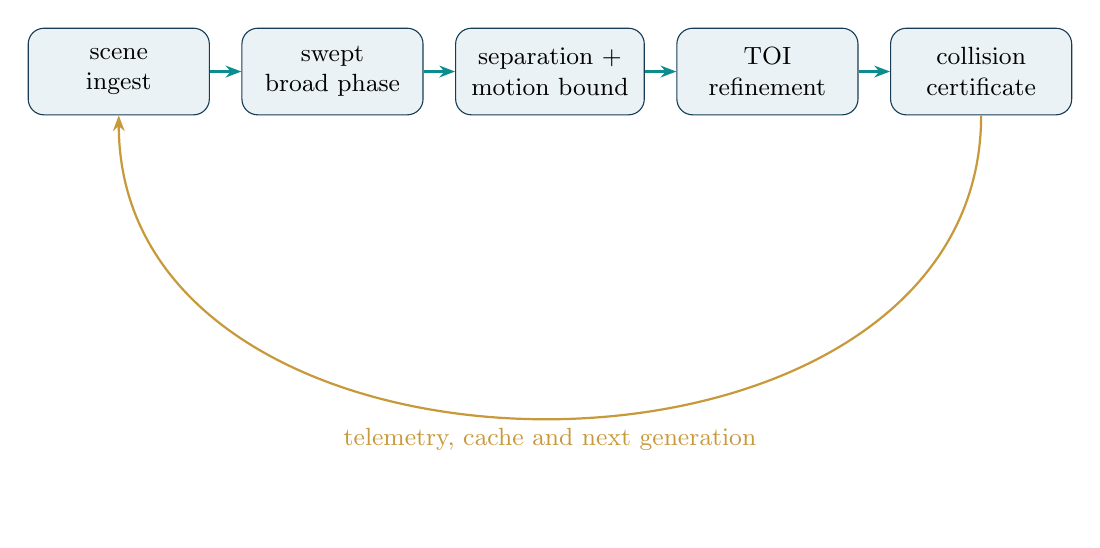
\begin{tikzpicture}[node distance=5mm and 4mm, every node/.style={font=\small,align=center}]
\tikzset{stage/.style={draw=nhdfnavy,rounded corners=2mm,fill=nhdflight,minimum width=23mm,minimum height=11mm,inner sep=2mm}}
\node[stage] (ingest) {scene\\ingest};
\node[stage,right=of ingest] (broad) {swept\\broad phase};
\node[stage,right=of broad] (bound) {separation +\\motion bound};
\node[stage,right=of bound] (refine) {TOI\\refinement};
\node[stage,right=of refine] (cert) {collision\\certificate};
\draw[-{Stealth[length=2mm]},thick,nhdfteal] (ingest)--(broad);
\draw[-{Stealth[length=2mm]},thick,nhdfteal] (broad)--(bound);
\draw[-{Stealth[length=2mm]},thick,nhdfteal] (bound)--(refine);
\draw[-{Stealth[length=2mm]},thick,nhdfteal] (refine)--(cert);
\draw[-{Stealth[length=2mm]},thick,nhdfgold] (cert.south) to[out=-90,in=-90,looseness=1.2] node[below]{telemetry, cache and next generation} (ingest.south);
\end{tikzpicture}
\end{center}

\vfill
\begin{decisionbox}[Release position]
This document turns the NHDF roadmap toward one falsifiable center: general-purpose continuous collision detection as an architecture, with an executable primitive reference and explicit pathways to robust mesh, convex, SDF, CPU, GPU, and application implementations. Optical, quantum, chemical, biological, medical, SAR, fabrication, and cosmological material is retained only through separate adapter contracts and evidence gates.
\end{decisionbox}
\vspace{8mm}
{\Large\bfseries Tom Klootwijk\par}
{\large 1 September 2026\par}
\vspace{4mm}
{\small Document status: research specification and executable validation scaffold. Not safety-certified, medically validated, cryptographically authoritative, or a claim that physical reality is an NHDF substrate.}
\end{titlepage}
\hypersetup{pageanchor=true}

\frontmatter
\chapter*{Document control}
\addcontentsline{toc}{chapter}{Document control}
\begin{tabularx}{\textwidth}{@{}L{0.24\textwidth}Y@{}}
\toprule
Field & Value \\
\midrule
Title & NHDF-CCD: CCD-Centered Formalization and Cradle-to-Grave Validation Dossier \\
Version & 0.4.0 \\
Author attribution & Tom Klootwijk \\
Date & 1 September 2026 \\
Primary center & Continuous Collision Detection (CCD) \\
Executable status & Python CPU reference; C++17 exact-sphere slice; CUDA source skeleton \\
Bundled verification & 22 Python tests, one C++ smoke test, four reference vectors, 5,000-query generated differential benchmark \\
Evidence class & Conceptual architecture plus bounded executable scaffold; no production or safety certification \\
Privacy rule & Civil identifiers and date of birth are not included in executable state or used as cryptographic material \\
\bottomrule
\end{tabularx}

\chapter*{Abstract}
\addcontentsline{toc}{chapter}{Abstract}
The supplied NHDF work develops an ordered vocabulary of log-polar addressing, local zero-level constraints, parity events, bounded branching, forward kinematics, analytic sweeps, projection, and feedback. The earlier formal specification made the essential non-degenerate correction that a global field satisfying $F\equiv 0$ is unusable and that each valid cell must instead lie on a nontrivial local constraint. The commute transcript then connected an SDF lookup and kinematic motion to Continuous Collision Detection, but overstated that connection as a complete one-clock solution. The whole-substrate extension mapped the vocabulary into sensors, actuators, chemistry, biology, medicine, photonics, quantum optics, fabrication, SAR, and cosmology.

Version 0.4 centers the research program on CCD because it supplies a precise mathematical question, exact and conservative reference methods, public benchmark datasets, explicit failure states, and a direct route from CPU semantics to GPU and application integration. A pairwise separation function $\sepfn(t)$ defines the contact zero set. Exact primitive solvers, conservative advancement, interval inclusion, swept broad-phase bounds, and bounded queues produce a certificate with one of seven states: \status{HIT}, \status{NO\_HIT}, \status{INITIAL\_OVERLAP}, \status{INCONCLUSIVE}, \status{UNSUPPORTED}, \status{INVALID\_INPUT}, or \status{CAPACITY\_EXCEEDED}. The NHDF log-polar, parity, golden-ratio, and topology constructs remain traceable as scheduling and experimental operators, but none may certify or suppress a collision unless an independent equivalence proof is established.

The accompanying package implements exact linear sphere--sphere, sphere--plane, and swept-AABB queries; conditional conservative advancement for declared separation oracles; point/sphere versus a true or conservatively bounded SDF under translation; a deterministic broad phase; interval-refinement ablations; schemas; telemetry; tests; benchmarks; a C++ slice; and a GPU plan. The remaining substrate materials are mapped through a uniform adapter contract that preserves domain-specific state, evolution laws, units, invariants, uncertainty, validation metrics, and stop conditions.

\chapter*{Executive determination}
\addcontentsline{toc}{chapter}{Executive determination}
\begin{decisionbox}[What this release establishes]
NHDF can be developed as a bounded, causal operator architecture around CCD. The scientifically defensible nucleus is the ordered closure of local constraints, kinematic prediction, conservative swept bounds, bounded refinement, observable certificates, and feedback telemetry. Version 0.4 makes that nucleus executable for a deliberately small primitive profile and gives every later implementation a testable contract.
\end{decisionbox}

\begin{warningbox}[What this release does not establish]
The release does not solve every possible CCD query, does not implement triangle-mesh or rotating-body robustness, does not include contact response, and does not demonstrate a GPU or physical-substrate advantage. It does not validate medical treatment, biological Cross-Kerr computation, universal golden-ratio branching, storm immunity, zero-latency optics, or cosmological holography. Those claims are either rejected or retained as separately gated hypotheses.
\end{warningbox}

\begin{gatebox}[Immediate next gate]
The next scientific milestone is not a larger vocabulary. It is robust differential validation against exact time-of-impact corpora and independent implementations for vertex--face and edge--edge triangle queries, followed by CPU/GPU equivalence. Only after that gate should an application claim be made.
\end{gatebox}

\tableofcontents
\listoffigures
\listoftables

\mainmatter

% =============================================================================
\part{Evidence boundary and architectural turn}
% =============================================================================

\chapter{Purpose, scope, and release philosophy}
\section{Why CCD becomes the center}
A useful research center must expose a clear input, a clear output, a correctness criterion, failure conditions, baselines, and a way to reproduce results. CCD satisfies all six. Given continuous object trajectories over a time interval, the engine must determine whether the objects first touch, identify or bound the earliest time, and avoid the tunneling failure of endpoint-only testing. Robust CCD research also provides exact or analytic datasets, inclusion-based algorithms, open implementations, and known degeneracies against which a new architecture can be tested \citep{wang2021tight,belgrod2023toi}.

The turn toward CCD does not discard the earlier NHDF work. It changes the burden of proof. Terms such as ``local zero set,'' ``forward timeline,'' ``bounded branch tree,'' and ``analytic sweep'' receive direct geometric meanings. Terms such as parity, golden-ratio scaling, and non-orientable chart flips are kept as optional scheduling or diagnostic variables until an ablation establishes their value. This preserves source traceability without allowing attractive vocabulary to substitute for a collision certificate.

\section{Cradle-to-grave means lifecycle, not only algorithm}
The package treats a collision engine as a lifecycle artifact:
\begin{enumerate}
  \item establish provenance and claim boundaries;
  \item define supported geometry, motion, units, tolerances, and hazards;
  \item formalize the mathematics and proof obligations;
  \item build a deterministic reference implementation;
  \item validate against exact and adversarial cases;
  \item port only verified semantics to accelerated hardware;
  \item integrate detection with a separate response solver and application policy;
  \item deploy with telemetry, incident replay, and explicit safe stops;
  \item maintain through controlled changes and regression evidence;
  \item retire unsafe or obsolete backends without silent degradation.
\end{enumerate}

Every stage in the ZIP has its own numbered directory. The PDF is therefore not the only product; it is the narrative and formal index to executable and operational artifacts.

\section{Authorship and privacy}
The work is attributed to Tom Klootwijk. Personal civil identifiers and dates of birth do not strengthen a mathematical proof, do not authenticate a runtime, and are not suitable cryptographic keys. The package intentionally omits them from executable state. Release authenticity should instead use repository history, reproducible builds, conventional digital signatures, and published hashes.

\chapter{Source register and claim disposition}
\section{Supplied materials}
The release is grounded in four supplied sources:
\begin{description}[leftmargin=2.2em,labelindent=0pt,labelsep=0.6em,font=\normalfont\bfseries]
  \item[S1 -- original operator-chain transcript.] A 30-page progression from parity, lower-case phi, log-polar LUT, kinematics, cone sweep, projections, distributed apex, BST/L-system branching, SDF/Klein-bottle language, and later GPU, optical, quantum, and SAR proposals \citep{source_prompt}.
  \item[S2 -- Formal Specification v0.1.] A 26-page formalization that separates NHDF representation, PCKF dynamics, and IHCP runtime; replaces the degenerate global zero field with cell-local constraints; distinguishes data and topology parity; bounds recursion; and defines a causal update \citep{source_formal01}.
  \item[S3 -- commute design transcript.] A 40-page design log that identifies the missing log-polar scale/Jacobian issue and then treats SDF plus kinematics as a claimed CCD solution, including collision-response bit operations and register-level metaphors \citep{source_commute}.
  \item[S4 -- spherical-Cartesian whole-substrate extension.] A 70-page extension into measurement, sensors, actuators, chemistry, biology, medicine, photonics, Cross-Kerr logic, microvasculature, lithography, direct writing, SAR, and cosmology \citep{source_substrate}.
\end{description}

\section{Four disposition classes}
\begin{tabularx}{\textwidth}{@{}L{0.18\textwidth}Y Y@{}}
\toprule
Class & Meaning & Example \\
\midrule
Preserved & The source idea already has a valid typed interpretation. & Monotonic forward time; bounded allocation; local zero-set residual. \\
Reinterpreted & The source insight is useful but its original mechanism or scope was too broad. & Parity becomes a hint or diagnostic rather than a universal collision governor. \\
Rejected & The statement conflicts with mathematics, physics, or the evidence available. & One SDF read and one sign-bit flip completely solve general CCD and collision response. \\
Adapter hypothesis & The idea may define a research program only after domain laws and validation are supplied. & Optical transfer, chemical event fields, biological waveguides, medical applications. \\
\bottomrule
\end{tabularx}

\section{The decisive corrections}
\subsection{From global zero to pairwise contact zero}
A global $F(x)\equiv 0$ has no distance or useful gradient. CCD instead uses a family of nontrivial pairwise separation functions,
\begin{equation}
  \sepfn(t)=\operatorname{sep}\big(A_i(t),B_j(t)\big),
  \qquad \mathcal{M}_{ij}=\{t\in[0,1]:\sepfn(t)=0\}.
\end{equation}
Positive separation means the pair is disjoint under the backend's convention; zero denotes contact; negative values denote overlap when a signed measure exists. This is the CCD-specific realization of distributed local zero-set semantics.

\subsection{From parity as physics to parity as bounded information}
A bitwise parity flag detects an odd count of bit inversions under a reference comparison and misses every even count. In a 2022 CCD paper, ``root parity'' is a precise mathematical construction for cubic roots, yet the authors explicitly note that parity cannot distinguish zero roots from the rare two-root case \citep{wang2022rootparity}. This is particularly instructive: parity can be valuable in CCD, but only with a clearly defined object and a known ambiguity. Version 0.4 therefore stores parity-derived scheduling metadata but never treats it as a complete collision predicate.

\subsection{From automatic logarithmic time dilation to coordinate-aware scheduling}
Log-polar coordinates can compact scale and convert rotation/scale relationships into shifts, but they do not increase physical sampling rate for free. The Jacobian and metric must be respected, and the underlying separation must remain coordinate invariant. Version 0.4 uses log-polar bins to group or prioritize work; it does not let a coordinate transform change whether two bodies collide.

\subsection{From a sign-bit response to a separate dynamics problem}
Collision detection answers when and where contact occurs. Response must use mass, inertia, normal, friction, restitution, constraints, compliance, and material failure. A sign inversion can be a toy elastic response in one dimension, not a general physical solver. The architecture therefore ends CCD at a certificate and hands that certificate to a separate response layer.

\small\begin{longtable}{@{}L{0.13\textwidth}L{0.23\textwidth}L{0.16\textwidth}L{0.38\textwidth}@{}}
\caption{Traceability from supplied sources to the v0.4 disposition.}\label{tab:traceability}\\
\toprule Source & Source idea & Disposition & v0.4 destination \\ \midrule
\endfirsthead
\toprule Source & Source idea & Disposition & v0.4 destination \\ \midrule
\endhead
S1 pp.1-6 & Parity-conditioned self-referential SDF engine & Reinterpreted & Local pair separation + bounded causal state; parity is diagnostic \\
S1 pp.8-11 & Operator precedence chain & Preserved with typing & State-threaded CCD chain and explicit address/candidate resolution \\
S1 pp.14-15 & Parity oscillation under disturbance & Preserved as failure signal & Debounce/telemetry/safe stop; no correction claim \\
S1 pp.16-18 & SDF zero in every LUT cell & Corrected & Family of nontrivial local constraints; in CCD, d\_ij(t)=0 \\
S1 pp.19-22 & Optical/quantum substrate & Separated & Operator-equivalence adapter only \\
S1 pp.22-30 & GPU/Tensor/VRAM claims & Corrected & Normal exposed operations, bounded queues, CPU equivalence first \\
S2 Sec.2-5 & Non-degenerate local zero sets & Adopted & Foundation for pairwise contact manifolds \\
S2 Sec.6-8 & Forward timeline, phase, bounded branching & Adopted with limitation & Causal TOI and bounded refinement; phase/golden are heuristic \\
S2 Sec.12 & GPU reference schedule & Extended & Broad/narrow phase, compaction, certificate emission \\
S3 pp.2-4 & Missing log-polar Jacobian & Preserved as coordinate warning & Coordinates may schedule work; geometry remains Cartesian/invariant \\
S3 pp.14-17 & SDF+kinematics completely solves CCD in one clock & Rejected & General CCD needs broad phase, robust narrow phase, TOI isolation, degeneracy handling, certificates \\
S3 pp.29-30 & Compare step magnitude with SDF & Partially adopted & Conditional conservative advancement with valid distance and speed bounds \\
S3 pp.31-36 & Autonomous/public-safety use & Restricted & Collision avoidance only, with governance; no identity or force decisions \\
S4 pp.12-18 & Universal sensors/actuators substrate & Separated & Measurement/actuation adapter with units and calibrated transfer laws \\
S4 pp.22-30 & Chemical, biological, macro, SAR, and cosmic maps & Separated & Independent adapters; no ontological unification \\
S4 pp.33-48 & Medical, microvascular, biophotonic, cross-Kerr claims & Rejected as therapeutic mechanism & Simulation/research hypotheses only \\
S4 pp.49-70 & Lithography, GDSII, 3D photonics & Separated & Fabrication adapter with PDK/DRC/metrology gates \\
\bottomrule
\end{longtable}

\chapter{Research context: what robust CCD actually requires}
\section{Broad phase and narrow phase}
Modern CCD systems separate a conservative broad phase from an accurate narrow phase. A false-negative broad phase is fatal because the narrow phase never sees the missed pair. Exact time-of-impact datasets have shown that implementation details can invalidate methods that appear correct on paper, and that broad and narrow phases must be evaluated together \citep{belgrod2023toi}. The v0.4 scaffold therefore treats candidate capacity and unsupported backends as visible states rather than silently dropping work.

\section{Families of methods}
The roadmap is backend-plural rather than method-monolithic:
\begin{itemize}
  \item \textbf{Closed-form primitive solvers} for spheres, planes, capsules, and translational boxes where stable roots or slabs are available.
  \item \textbf{Conservative advancement} for convex or implicit geometry when a trustworthy distance and motion bound exist \citep{mirtich1996,zhang2006}.
  \item \textbf{Interval and inclusion methods} for robust polynomial or parametric-surface queries \citep{wang2021tight,chen2024tdibm}.
  \item \textbf{Feature-based mesh CCD} using vertex--face and edge--edge tests, exact predicates, degeneracy handling, and adjacency filters.
  \item \textbf{Contact-integrated methods} such as IPC and its codimensional/rigid variants, which depend on collision queries but also solve a larger time-stepping problem \citep{li2021cipc,ferguson2021rigidipc}.
  \item \textbf{SDF-specific methods}. Recent work treats triangle--SDF contact directly and, in 2026, SDF--SDF time of impact through alternating spatial-temporal optimization \citep{pelletier2025trisdf,nielsen2026sdfsdf}.
  \item \textbf{Convex cone/ray casting and hardware acceleration}. C5D and GPU ray-tracing research illustrate active directions without implying that one representation dominates every workload \citep{yuan2025c5d,sui2024rtccd}.
\end{itemize}

\section{The reference does not compete with those methods yet}
The bundled Python implementation is intentionally modest. It validates the state machine, certificate semantics, conservative-advance proof obligation, failure preservation, deterministic traces, and lifecycle tooling. It is not presented as a replacement for Tight Inclusion, IPC Toolkit, or a production physics engine. Those projects supply the correct next comparison points; IPC Toolkit itself exposes broad- and narrow-phase CCD for linear and nonlinear trajectories and explicitly states that it is not a complete physics solver \citep{ipctoolkit}.

% =============================================================================
\part{CCD formal core}
% =============================================================================

\chapter{Problem statement and outcome semantics}
\section{Scene and motion}
Let a scene contain bodies $B_i=(S_i,M_i)$, where $S_i$ is a geometric shape and $M_i$ maps normalized step time $t\in[0,1]$ to a configuration. The normalized interval avoids binding the mathematics to a particular frame duration; physical time is recovered by $\tau=\tau_n+t\Delta\tau_n$.

For a pair $(i,j)$, a narrow-phase backend provides or derives:
\begin{enumerate}
  \item a separation or inclusion object $\sepfn(t)$;
  \item witness features or points when meaningful;
  \item a contact normal or normal set when meaningful;
  \item a conservative bound on change over an interval;
  \item a procedure for isolating the earliest contact.
\end{enumerate}

The first time of impact is
\begin{equation}
  \TOI = \inf\{t\in[0,1]:\sepfn(t)\le 0\},
\end{equation}
with conventions adjusted for a minimum separation or thickness. If the pair overlaps at $t=0$, the query is not reported as an ordinary future hit.

\section{Seven outcomes}
\begin{longtable}{@{}L{0.22\textwidth}L{0.30\textwidth}L{0.38\textwidth}@{}}
\caption{Normative certificate outcomes.}\label{tab:statuses}\\
\toprule Status & Meaning & Caller permission and obligation \\ \midrule
\endfirsthead
\toprule Status & Meaning & Caller permission and obligation \\ \midrule
\endhead
\status{HIT} & Contact is found within the interval. Exact backends return a point; iterative backends return a conservative bracket. & Advance no later than the certified upper TOI, group simultaneous contacts, and invoke response. \\
\status{NO\_HIT} & The supported backend certifies positive separation throughout the interval. & The caller may advance through the step for that pair. \\
\status{INITIAL\_OVERLAP} & Separation is negative at the start. & Roll back, depenetrate, or invoke a dedicated overlap solver. Do not pretend the overlap began later. \\
\status{INCONCLUSIVE} & A possible contact could not be safely classified within numerical or resource bounds. & Reduce the step, increase precision/budget, or switch backend. \\
\status{UNSUPPORTED} & No declared backend covers the shape/motion pair. & Route to another backend or reject the scene. \\
\status{INVALID\_INPUT} & A value, tolerance, bound, or oracle contract is invalid. & Quarantine the query and fail safe. \\
\status{CAPACITY\_EXCEEDED} & A bounded pool or queue could not contain required work. & Preserve the required count and reconfigure; never reinterpret as no-hit. \\
\bottomrule
\end{longtable}

\section{Collision certificate}
A certificate is the minimum auditable output:
\begin{equation}
\mathcal{C}_{ij}=\big(s, [t^-,t^+], \mathcal{W}, n, b, k, \mathcal{T}, h\big),
\end{equation}
where $s$ is status, $[t^-,t^+]$ is the TOI bracket, $\mathcal{W}$ contains witnesses, $n$ is a normal, $b$ names the backend, $k$ is iteration count, $\mathcal{T}$ is bounded telemetry, and $h$ is a deterministic digest. The digest is for replay integrity, not a replacement for a signed release or evidence chain.

\chapter{Typed, state-threaded operator chain}
\section{Why the older composition needed repair}
The v0.1 chain correctly ordered log-polar encoding, local boundary projection, parity, routing, kinematics, sweep, projection, and update. Its written function signatures, however, did not literally compose: an address is not a candidate cell, a bit is not a branch tree, and a tree is not a trajectory. Version 0.4 threads one enriched state through each stage.

\section{Common state}
\begin{align}
\SigmaState = (&\mathcal{S}, I_t, \mathcal{B}, \mathcal{P}, \mathcal{O}, \mathcal{Q},
\mathcal{C}, \mathcal{H}, \mathcal{F}),
\end{align}
where $\mathcal{S}$ is the scene, $I_t$ the active time interval, $\mathcal{B}$ swept bounds, $\mathcal{P}$ candidate pairs, $\mathcal{O}$ separation oracles, $\mathcal{Q}$ bounded refinement queues, $\mathcal{C}$ certificates, $\mathcal{H}$ telemetry/history, and $\mathcal{F}$ failures.

Every operator has type $O_k:\Sigma\rightarrow\Sigma$. The normative chain is
\begin{equation}
\boxed{
\Sigma' = U\circ\Pi_{\mathrm{cert}}\circ R_{\mathrm{refine}}\circ A_{\mathrm{CA}}
\circ B_{\mathrm{bound}}\circ C_{\mathrm{pair}}\circ E_{\mathrm{scene}}(\Sigma)
}
\end{equation}
with optional source-traceable scheduling metadata $H_{\mathrm{NHDF}}$ that may modify priority but not classification.

\begin{figure}[H]
\centering
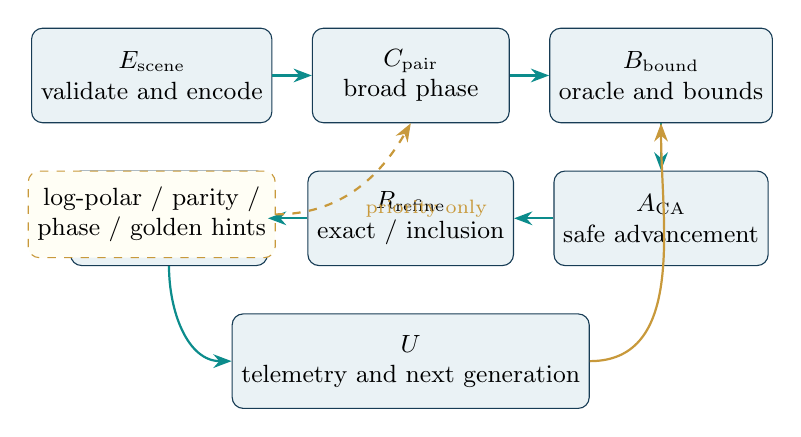
\begin{tikzpicture}[node distance=6mm and 5mm, every node/.style={font=\small,align=center}]
\tikzset{op/.style={draw=nhdfnavy,rounded corners,fill=nhdflight,minimum width=25mm,minimum height=12mm}, hint/.style={draw=nhdfgold,dashed,rounded corners,fill=yellow!4,minimum width=28mm,minimum height=11mm}}
\node[op] (e) {$E_{\rm scene}$\\validate and encode};
\node[op,right=of e] (c) {$C_{\rm pair}$\\broad phase};
\node[op,right=of c] (b) {$B_{\rm bound}$\\oracle and bounds};
\node[op,below=of b] (a) {$A_{\rm CA}$\\safe advancement};
\node[op,left=of a] (r) {$R_{\rm refine}$\\exact / inclusion};
\node[op,left=of r] (p) {$\Pi_{\rm cert}$\\emit certificate};
\node[op,below=of r] (u) {$U$\\telemetry and next generation};
\node[hint,below=of e] (h) {log-polar / parity /\\phase / golden hints};
\draw[-{Stealth},thick,nhdfteal] (e)--(c);
\draw[-{Stealth},thick,nhdfteal] (c)--(b);
\draw[-{Stealth},thick,nhdfteal] (b)--(a);
\draw[-{Stealth},thick,nhdfteal] (a)--(r);
\draw[-{Stealth},thick,nhdfteal] (r)--(p);
\draw[-{Stealth},thick,nhdfteal] (p.south) to[out=-90,in=180] (u.west);
\draw[-{Stealth},thick,nhdfgold,dashed] (h.east) to[out=0,in=-120] node[below right,font=\scriptsize]{priority only} (c.south);
\draw[-{Stealth},thick,nhdfgold] (u.east) to[out=0,in=-90] (b.south);
\end{tikzpicture}
\caption{State-threaded CCD chain. Dashed NHDF hints are deliberately outside the correctness authority.}
\label{fig:typed-chain}
\end{figure}

\section{Operator obligations}
\begin{tabularx}{\textwidth}{@{}L{0.16\textwidth}Y Y@{}}
\toprule
Operator & Must produce & Must never do \\
\midrule
$E_{\rm scene}$ & Valid units, finite values, normalized time, declared shape and motion profiles. & Silently clamp invalid values into apparently valid geometry. \\
$C_{\rm pair}$ & Conservative candidates and explicit overflow. & Prune on an unverified learned, parity, or log-polar heuristic. \\
$B_{\rm bound}$ & A backend contract: distance/inclusion object, witnesses, and valid motion/error bounds. & Call an approximate field a signed distance without a conservative error envelope. \\
$A_{\rm CA}$ & Certified no-skip time advances or an explicit stall/failure. & Force a minimum step larger than the safe bound. \\
$R_{\rm refine}$ & Earliest-contact isolation under exact, interval, or conservative semantics. & Convert budget exhaustion into no-hit. \\
$\Pi_{\rm cert}$ & Complete status, bracket, backend, tolerance, trace, and digest. & Hide initial overlap or unsupported geometry. \\
$U$ & Deterministic state/telemetry update. & Change a geometric result after certification. \\
\bottomrule
\end{tabularx}

\chapter{Exact primitive backends}
\section{Linear sphere--sphere}
Let $p=c_B(0)-c_A(0)$, $v=v_B-v_A$, and $R=r_A+r_B$. Contact solves
\begin{equation}
  \|p+tv\|^2=R^2,
\end{equation}
which yields $at^2+bt+c=0$ with
\begin{equation}
  a=v\cdot v,\qquad b=2p\cdot v,\qquad c=p\cdot p-R^2.
\end{equation}
The earliest root in $[0,1]$ is the TOI. The implementation checks initial overlap before root solving and uses a stable quadratic formulation. This exact backend is the main ground truth for the bundled randomized benchmark.

\section{Linear sphere--plane}
For a one-sided plane $n\cdot x=o$ and a sphere center $c(t)$,
\begin{equation}
  d(t)=n\cdot c(t)-o-r.
\end{equation}
Under linear relative translation, $d$ is linear. A negative initial value is overlap; a nonnegative derivative while $d(0)>0$ is a no-hit certificate; otherwise $t=-d(0)/\dot d$.

\section{Swept axis-aligned boxes}
For each axis, relative box centers and summed half-extents produce a one-dimensional overlap interval. The boxes collide if and only if the three slab intervals overlap in time. The maximum entry time is the TOI and identifies an entry normal. The backend is exact only while the boxes remain axis-aligned and motion is translational linear.

\section{Why exact primitives matter in a general architecture}
A general engine should not force every query through one iterative method. Closed-form or slab solutions are cheaper, easier to validate, and excellent differential oracles. Version 0.4 therefore dispatches by typed pair and motion profile before using conservative advancement.

\chapter{Conservative advancement as the SDF bridge}
\section{The useful part of the source intuition}
The commute transcript's central CCD intuition is recognizable: if the current distance is trustworthy and the maximum rate of closure is bounded, the engine may advance by a fraction of distance divided by speed without passing through contact. This is conservative advancement, not a new one-clock law \citep{mirtich1996,zhang2006}.

\section{No-skip theorem}
Assume $d:[a,b]\rightarrow\R$ is continuous and $L$-Lipschitz,
\begin{equation}
 |d(t)-d(s)|\le L|t-s|,
\end{equation}
where $d(t)>0$ denotes separation. At time $t_k$, choose
\begin{equation}
 h_k=\eta\frac{d(t_k)}{L_k},\qquad 0<\eta\le 1,
\end{equation}
with $L_k$ valid on the interval to be covered. For any $0\le s<h_k$,
\begin{equation}
 d(t_k+s)\ge d(t_k)-L_ks > d(t_k)(1-\eta)\ge 0.
\end{equation}
Thus the open interval is collision-free. Repeated safe advances cannot skip a first contact, provided the distance is not overestimated and the speed bound is not underestimated.

\begin{warningbox}[The two contracts that cannot be waived]
A sampled texture, neural implicit field, approximate Euclidean distance transform, or interpolated SDF may overestimate true separation. A velocity bound that ignores rotation, deformation, acceleration, or calibration error may underestimate closure. Either violation destroys the no-skip guarantee. In that case the engine must add a conservative bias/error bound or return \status{UNSUPPORTED}/\status{INCONCLUSIVE}.
\end{warningbox}

\section{SDF specialization}
For a true signed distance $F$ with spatial Lipschitz constant 1 and a moving point $x(t)$ with $\|\dot x\|\le V$, the composed separation $d(t)=F(x(t))-r$ is $V$-Lipschitz. If the field moves, a conservative relative-speed bound is used. If the field's Lipschitz bound is $K$, then $L\le K V_{\rm rel}$. The executable reference supports point/sphere versus an implicit field under translation through exactly this contract.

\section{Termination and brackets}
The reference stops when distance is within a declared tolerance and returns the previous and current sample as a conservative contact bracket. If the safe step falls below temporal resolution before the distance tolerance is reached, the result is \status{INCONCLUSIVE}; it does not force a larger step. If the current distance minus the speed bound times remaining time stays positive, the algorithm returns a no-hit certificate for the rest of the interval.

\begin{figure}[H]
\centering
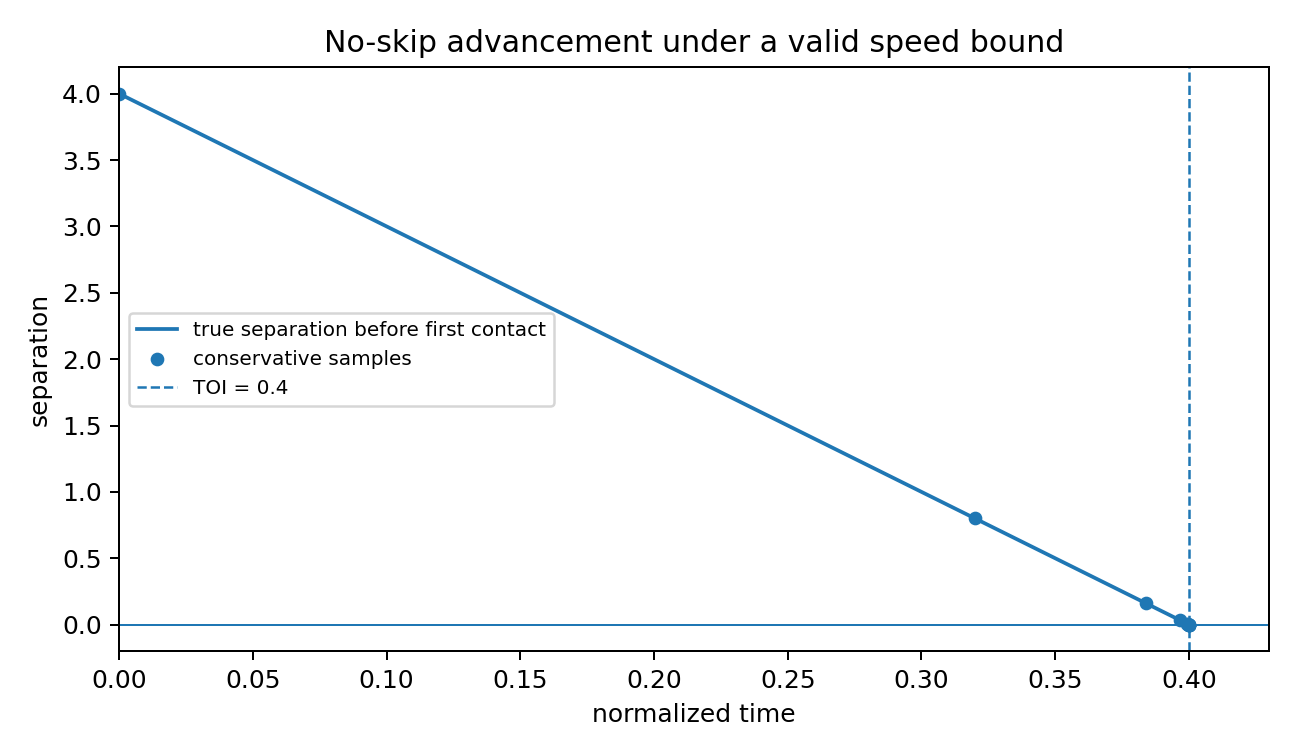
\includegraphics[width=0.86\textwidth]{figures/conservative_trace.png}
\caption{Reference conservative advancement toward a unit-sphere SDF. Sample spacing contracts near contact; no free ``time dilation'' is claimed.}
\label{fig:ca-trace}
\end{figure}

\section{Pseudocode}
\begin{lstlisting}[language=Python,caption={Semantics of conservative advancement in v0.4.}]
sample = oracle.evaluate(t)
if sample.distance < -distance_tolerance:
    return INITIAL_OVERLAP
if sample.distance <= distance_tolerance:
    return HIT at t

while budget remains:
    L = oracle.closure_speed_bound(t, t_end)
    if L <= speed_epsilon:
        return NO_HIT
    if sample.distance - L * (t_end - t) > 0:
        return NO_HIT with remaining-interval certificate
    h = safety_factor * sample.distance / L
    if h <= time_tolerance:
        return INCONCLUSIVE
    previous_t = t
    t = t + h
    sample = oracle.evaluate(t)
    if sample.distance <= distance_tolerance:
        return HIT bracket [previous_t, t]
return INCONCLUSIVE
\end{lstlisting}

\chapter{Broad phase and bounded work}
\section{Conservative swept bounds}
For a body with translational motion, each coordinate is bounded over the step, including a quadratic extremum where velocity crosses zero. Shape extents expand that center interval into a swept AABB. A sweep-and-prune pass sorts by minimum $x$, maintains an active list, and tests overlap on all axes. Infinite planes are conservatively paired with bounded bodies.

\section{Capacity is part of semantics}
A finite machine has finite candidates, nodes, trace records, and output capacity. Let $N_c$ be generated candidates and $N_c^{\max}$ the configured capacity. The invariant is not ``overflow cannot happen''; it is
\begin{equation}
 N_c\le N_c^{\max}\quad\text{or the result is }\status{CAPACITY\_EXCEEDED}.
\end{equation}
A silent truncation would be indistinguishable from a false-negative broad phase.

\section{Bounded interval refinement and the BST mapping}
The source BST/L-system becomes a bounded earliest-first refinement tree. For interval $I=[a,b]$, sample the midpoint $m$ and use a valid Lipschitz bound $L_I$:
\begin{equation}
 \underline d(I)=d(m)-\frac{L_I}{2}(b-a).
\end{equation}
If $\underline d(I)>0$, the interval is collision-free. Otherwise it is sampled or subdivided until contact, certification, time tolerance, or node capacity. The split may be midpoint or a golden-ratio point as an experiment. The lower bound, not the aesthetic of the tree, supplies correctness.

\section{Branching ablation rule}
The golden-ratio policy \must be compared with midpoint, adaptive, and backend-specific policies at equal node budget. If it does not improve a predeclared metric, it remains a source-traceable curiosity rather than a justified operator.

\chapter{Log-polar, phase, parity, and topology in the CCD profile}
\section{Log-polar hint}
The reference computes scheduling metadata from nonnegative separation and relative approach direction,
\begin{equation}
 \rho=\log(1+d),\qquad \theta=\operatorname{atan2}(v_y,v_x),
\end{equation}
quantizes $(\rho,\theta,t)$, packs a word, and records its bit parity. A priority such as $(d+\epsilon)^{-1}$ can place near contacts earlier in a work queue. The hint can improve coherence or load balance; it cannot delete a pair or certify no-hit.

\section{Second phase difference}
For a directional phase sequence $\phi_n$, the source's $\Delta\Delta\phi$ becomes
\begin{equation}
 \Delta^2\phi_n=\operatorname{wrap}(\phi_n-2\phi_{n-1}+\phi_{n-2}).
\end{equation}
It may predict rapidly changing approach direction and request a stronger backend or smaller global step. It is not a bound unless a separate derivation relates it to motion.

\section{Parity firewall}
\begin{decisionbox}[Normative parity firewall]
Enabling or disabling NHDF parity/log-polar hints must not change the supported collision classification or certificate validity. It may change query order, iteration budget escalation, diagnostics, or performance. The bundled test suite checks classification invariance for the SDF example.
\end{decisionbox}

\section{Klein-bottle topology}
A Klein-bottle quotient can model non-orientable chart transitions in a specialized geometry system, but ordinary Euclidean collision detection does not require it. If a simulation explicitly uses a non-orientable manifold, chart metadata must be handled by the geometry backend. An orientation flip is not equivalent to a payload error, collision, or response impulse.

\chapter{Contact output and the boundary with response}
\section{Witnesses and normals}
A hit certificate may carry points $w_A,w_B$ and a normal $n$. For sphere--sphere contact, $n$ follows the center difference and the witnesses lie at radii along the normal. For implicit fields, the gradient supplies a local normal only if it is well-conditioned and consistent with the field's sign convention. Degenerate or multiple contacts may require a normal set or contact manifold rather than one vector.

\section{Simultaneous contacts}
Let $t_*$ be the earliest upper TOI across pairs. A response layer should group all contacts satisfying
\begin{equation}
 t^-_{ij}\le t_*+\tau_{\rm group}
\end{equation}
under a declared tolerance. Processing one pair and advancing past another simultaneous contact can create order-dependent penetrations.

\section{Detection is not response}
A frictionless point-mass reflection may use
\begin{equation}
 v^+ = v^- -(1+e)(v^-\cdot n)n,
\end{equation}
for restitution $e$, but rigid bodies require angular momentum and effective mass; friction needs tangential constraints; resting contact and stacking need persistent constraints or potentials; deformable bodies need constitutive models. CCD supplies the event and geometry, not these laws.

\begin{figure}[H]
\centering
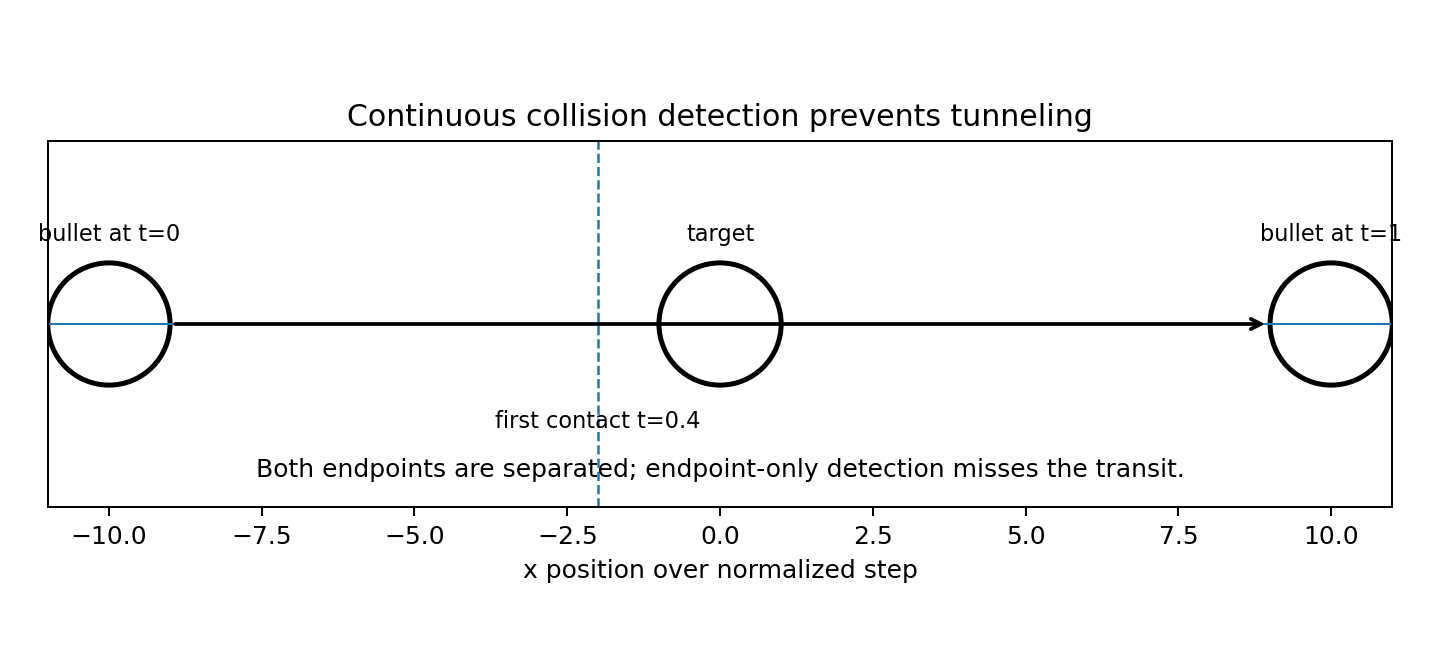
\includegraphics[width=0.92\textwidth]{figures/tunneling_demo.png}
\caption{A sphere can cross another sphere while both frame endpoints remain separated. CCD isolates the first contact instead of responding to an already penetrated final state.}
\label{fig:tunneling}
\end{figure}

% =============================================================================
\part{Executable reference and verification}
% =============================================================================

\chapter{Reference implementation architecture}
\section{Package structure}
\begin{tabularx}{\textwidth}{@{}L{0.26\textwidth}Y@{}}
\toprule
Module & Responsibility \\
\midrule
\texttt{vector.py} & Minimal deterministic three-dimensional vector operations. \\
\texttt{motion.py} & Static, linear, and quadratic translational motion with speed and coordinate bounds. \\
\texttt{shapes.py} & Sphere, axis-aligned box, plane, point, and implicit-SDF types. \\
\texttt{oracles.py} & Separation samples, witnesses, normals, and closure-speed bounds. \\
\texttt{exact.py} & Exact linear primitive backends. \\
\texttt{conservative.py} & Contract-driven conservative advancement. \\
\texttt{interval.py} & Bounded midpoint/golden interval-refinement ablation. \\
\texttt{broadphase.py} & Swept bounds and deterministic sweep-and-prune. \\
\texttt{nhdf.py} & Log-polar, parity, and phase scheduling metadata outside the safety path. \\
\texttt{engine.py} & Typed dispatch and scene-level status reduction. \\
\texttt{types.py} & Configuration, status, samples, certificates, scene results, and trace hashes. \\
\texttt{io.py}/\texttt{cli.py} & Serialized scene loading and command-line execution. \\
\bottomrule
\end{tabularx}

\section{Design principles embodied in code}
\begin{enumerate}
  \item \textbf{Dispatch before iteration.} Exact profiles are selected before generic advancement.
  \item \textbf{Contracts are visible.} SDF Lipschitz and conservative-bias values are explicit fields.
  \item \textbf{No hidden allocation.} Candidate capacity and trace capacity are bounded.
  \item \textbf{No hidden fallback.} Unsupported pairs remain \status{UNSUPPORTED}.
  \item \textbf{Deterministic replay.} A canonical JSON trace is hashed with SHA-256.
  \item \textbf{Hints cannot decide.} NHDF metadata is attached after sampling and does not change the geometry path.
\end{enumerate}

\section{Exact sphere implementation excerpt}
\lstinputlisting[language=Python,firstline=19,lastline=75,caption={Exact linear sphere--sphere backend from the bundled Python reference.}]{../03_reference_implementation/python/src/nhdf_ccd/exact.py}

\section{Conservative implementation excerpt}
\lstinputlisting[language=Python,firstline=8,lastline=95,caption={Beginning of the conservative-advancement implementation, including explicit stall and invalid-bound behavior.}]{../03_reference_implementation/python/src/nhdf_ccd/conservative.py}

\section{C++ and GPU slices}
The C++17 directory implements the exact sphere--sphere query and builds without external dependencies. The CUDA directory contains a source-only batched exact sphere kernel. It was not compiled in the release environment because no CUDA compiler or target GPU was available. The report therefore makes no CUDA performance or equivalence claim.

\chapter{Test plan and included results}
\section{Test layers}
The package contains 22 Python tests spanning exact roots, high-speed tunneling, no-hit, initial overlap, AABB slabs, true-SDF conservative advancement, sphere radius against an SDF, quadratic translation, invalid Lipschitz values, hint invariance, interval split policies, broad-phase pruning, capacity failure, unsupported pairs, deterministic digests, and invalid configuration. A C++ smoke test independently checks the sphere--sphere TOI.

\section{Generated differential benchmark}
The reproducible benchmark generates \BenchQueries{} linear sphere--sphere queries with a fixed seed. The exact quadratic backend is treated as ground truth and compared with the conservative-advancement oracle. It also evaluates a deliberately weak detector that checks only $t=0$ and $t=1$.

\begin{table}[H]
\centering
\caption{Bundled generated benchmark summary. Timings are machine-specific CPython measurements and not product claims.}
\begin{tabular}{@{}lr@{}}
\toprule
Metric & Result \\
\midrule
Queries & \BenchQueries \\
Exact hits & \BenchHits \\
Hits missed by endpoint-only discrete check & \BenchEndpointMisses \\
Conservative false negatives & \BenchFalseNegatives \\
Conservative false positives & \BenchFalsePositives \\
Conservative inconclusive & \BenchInconclusive \\
Mean / maximum CA iterations & \BenchMeanIterations{} / \BenchMaxIterations \\
Mean TOI upper error & \BenchMeanToiError \\
Maximum TOI upper error & \BenchMaxToiError \\
Exact / CA queries per second & \BenchExactQps{} / \BenchCaQps \\
\bottomrule
\end{tabular}
\end{table}

\begin{figure}[H]
\centering
\begin{subfigure}{0.49\textwidth}
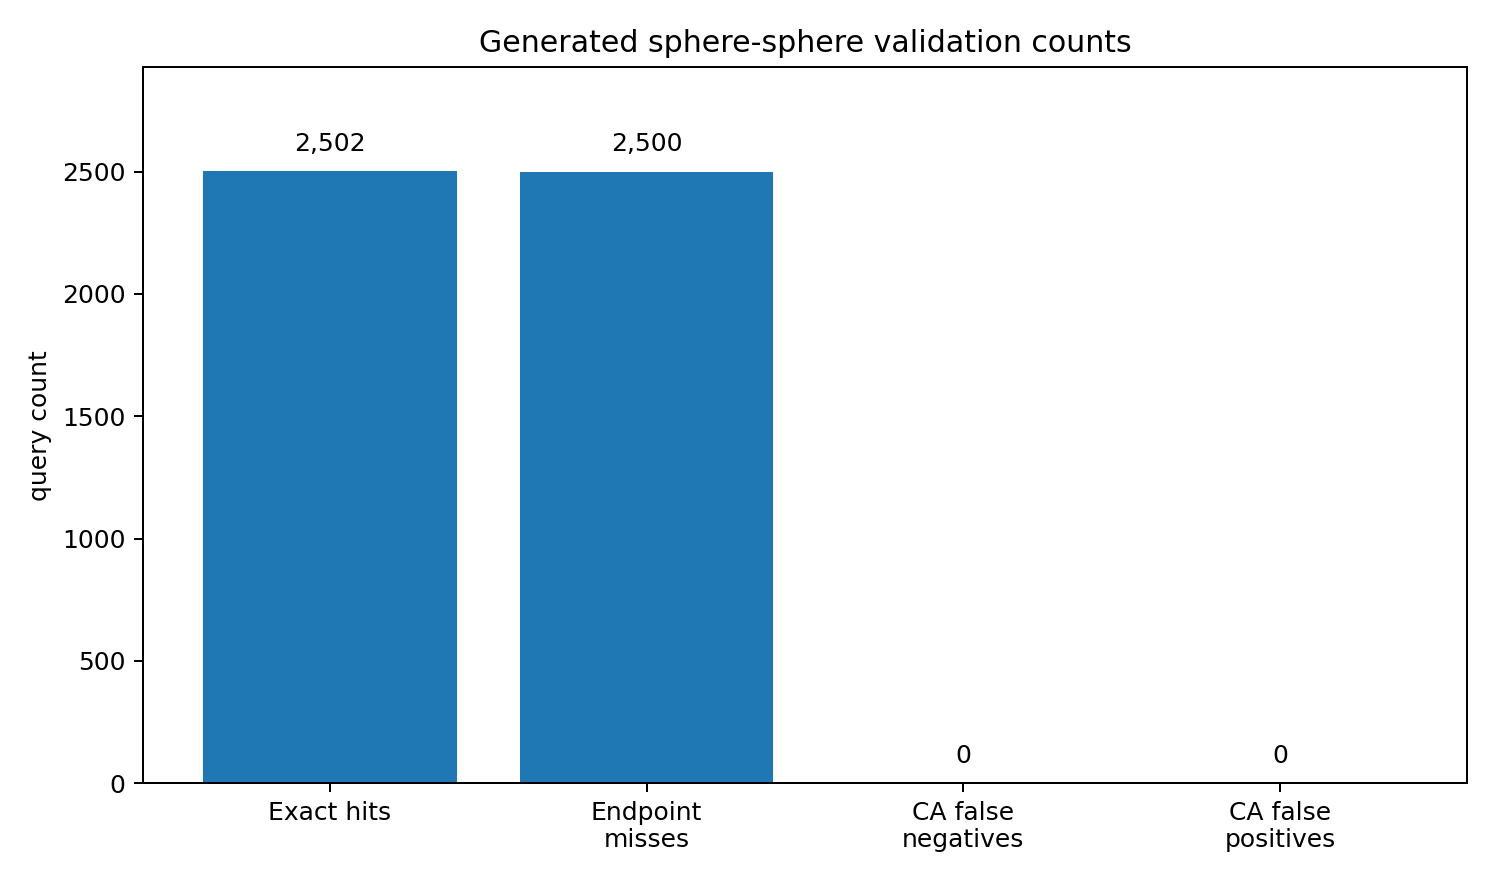
\includegraphics[width=\textwidth]{figures/benchmark_correctness.png}
\caption{Classification counts.}
\end{subfigure}\hfill
\begin{subfigure}{0.49\textwidth}
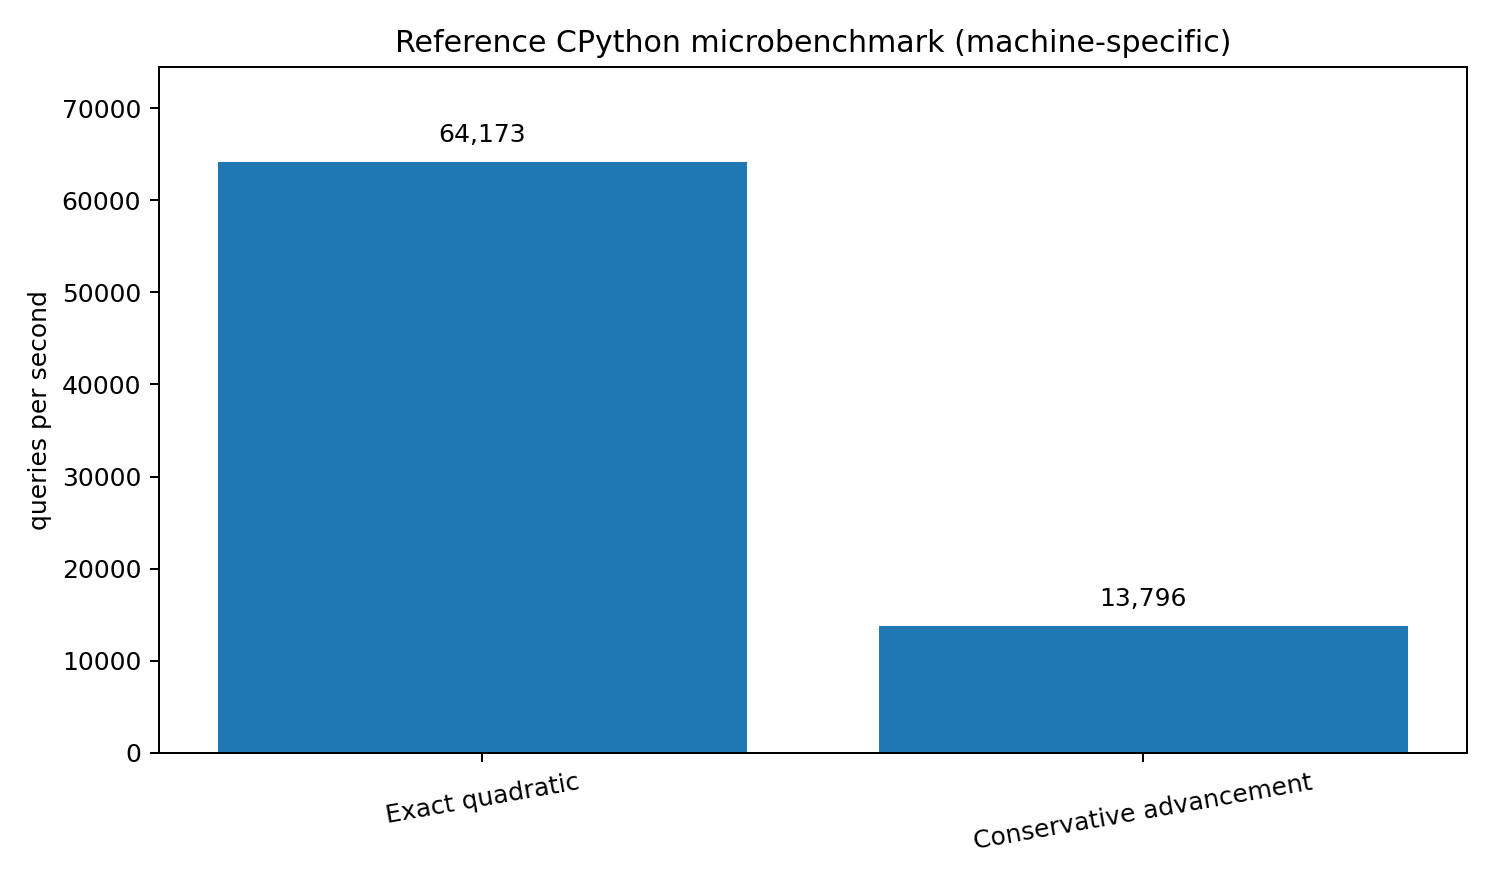
\includegraphics[width=\textwidth]{figures/benchmark_throughput.png}
\caption{Reference throughput.}
\end{subfigure}
\caption{The benchmark verifies the included sphere profile and demonstrates the endpoint-tunneling failure. It does not validate mesh or GPU completeness.}
\label{fig:benchmark}
\end{figure}

\section{Interpretation}
The zero false-negative result is evidence that the implementation matches its exact oracle on this generated distribution. It is not a statistical proof over all inputs. The next gate must use exact corpora containing millions of realistic and near-degenerate feature queries, as advocated by the CCD benchmark literature \citep{wang2021tight,belgrod2023toi}.

\chapter{Robustness and adversarial validation plan}
\section{Mandatory geometry cases}
\begin{enumerate}
  \item tangential contact and repeated roots;
  \item near-parallel edge--edge and near-coplanar vertex--face motion;
  \item contact at exactly $t=0$ or $t=1$;
  \item zero-area triangles, duplicate vertices, and zero-length edges;
  \item coincident features and ambiguous normals;
  \item scale extremes and mixed units;
  \item rapidly rotating shapes whose closest feature changes;
  \item accelerated and nonlinear trajectories;
  \item adjacency and self-collision filters;
  \item multiple simultaneous impacts.
\end{enumerate}

\section{Mandatory software and resource cases}
\begin{enumerate}
  \item NaN, infinity, signed zero, overflow, underflow, and denormal behavior;
  \item compiler and optimization differences;
  \item deterministic tie ordering;
  \item candidate, queue, trace, and output exhaustion;
  \item stale generation reads and ring-buffer wrap;
  \item CPU/GPU disagreement;
  \item corrupted serialized scenes and invalid schemas;
  \item approximate SDFs with known positive and negative error.
\end{enumerate}

\section{Differential program}
Version 0.5 should ingest public exact TOI data and compare at least three independent paths: an exact/inclusion reference, the NHDF-CCD backend under test, and a second established library. It should report false negatives, false positives, TOI interval width, runtime distribution, memory, and failure status by case family. Test results should remain linked to release and compiler hashes.

\chapter{Falsifiable NHDF hypotheses inside CCD}
\section{Core hypotheses}
\begin{longtable}{@{}L{0.10\textwidth}L{0.48\textwidth}L{0.32\textwidth}@{}}
\caption{CCD-centered falsifiable hypotheses.}\label{tab:hypotheses}\\
\toprule ID & Hypothesis & Required comparison \\ \midrule
\endfirsthead
\toprule ID & Hypothesis & Required comparison \\ \midrule
\endhead
H-CCD-1 & Log-polar bins reduce divergence or improve cache/work-queue locality without changing classification. & Equal queries, equal backend, linear/Cartesian or distance-only bucketing. \\
H-CCD-2 & A parity-derived anomaly signal predicts queries that require escalation. & Threshold, residual magnitude, random bit, and no-hint baselines; ROC and cost. \\
H-CCD-3 & $\Delta^2\phi$ improves motion-bound selection for rapidly changing approach direction. & Actual orientation/curvature bounds and fixed conservative bounds. \\
H-CCD-4 & Golden-ratio interval splitting reduces nodes or time for a declared workload. & Midpoint, secant, adaptive, and earliest-first strategies at equal correctness. \\
H-CCD-5 & Bounded self-referential feedback improves next-frame broad-phase coherence. & Open-loop refit/rebuild and standard temporal coherence baselines. \\
H-CCD-6 & SDF-specific backends improve quality-per-cost for complex implicit geometry. & Triangle mesh, convex proxy, and recent triangle--SDF/SDF--SDF methods. \\
H-CCD-7 & GPU implementation preserves all CPU statuses and TOI bounds while improving throughput or latency. & Deterministic replay on exact and adversarial corpora. \\
\bottomrule
\end{longtable}

\section{Kill criteria}
An NHDF-specific operator should be removed from the CCD path when it fails equal-budget ablations, increases false negatives, widens TOI bounds without compensating value, creates excessive divergence, or cannot be explained independently of the source metaphor. The architecture is stronger when unnecessary operators are deleted.

% =============================================================================
\part{Hardware, integration, and lifecycle}
% =============================================================================

\chapter{GPU roadmap}
\section{Semantics first}
GPU acceleration begins only after a CPU backend passes exact differential tests. The GPU is not asked to execute ``topology'' or ``SDF zero'' by name; it executes concrete bounds, roots, interval predicates, scans, queues, distance queries, and reductions. Matrix or ray hardware is used only where exposed semantics match the subproblem.

\section{Proposed pipeline}
\begin{enumerate}
  \item upload or generate structure-of-arrays body state;
  \item compute swept bounds;
  \item run a conservative broad phase;
  \item compact candidates with prefix sums while returning required count and overflow;
  \item bucket by backend and motion type;
  \item execute batched exact primitive kernels;
  \item execute robust mesh/inclusion work queues;
  \item reduce earliest TOI with a deterministic tie policy;
  \item emit certificates and bounded traces;
  \item replay selected samples on CPU.
\end{enumerate}

\section{Floating-point policy}
Fast-math modes can alter predicate signs and root intervals. The GPU profile must classify operations into performance-tolerant arithmetic and correctness-critical predicates. A faster kernel that silently changes \status{HIT} to \status{NO\_HIT} is not an optimization. Exact/inclusion methods and outward rounding may be required for robust backends.

\section{NHDF scheduling experiments}
Log-polar separation/approach bins could group similar iteration counts; $\Delta^2\phi$ could identify changing motion; parity could request replay; golden splits could shape work queues. Each experiment must preserve the candidate set and certificate semantics. The source CUDA/Tensor claims are therefore replaced by measurable scheduling hypotheses rather than assertions that Tensor Cores implement parity or topology.

\section{Acceptance metrics}
\begin{itemize}
  \item zero false negatives on declared exact corpora;
  \item CPU/GPU status equality;
  \item TOI bracket containment and width;
  \item overflow and unsupported-state equality;
  \item latency percentiles, not only average throughput;
  \item memory and queue high-water marks;
  \item energy and thermal behavior on the actual device;
  \item deterministic mode and documented non-deterministic high-throughput mode.
\end{itemize}

\chapter{Application integration and response boundary}
\section{Step protocol}
A conservative event-driven simulation step is:
\begin{enumerate}
  \item predict but do not commit motion;
  \item find candidates and query CCD;
  \item select the earliest conservative TOI;
  \item group near-simultaneous contacts;
  \item advance to the allowed time;
  \item solve response or constraints;
  \item repeat for the remaining substep under a bounded event count;
  \item commit state and telemetry.
\end{enumerate}

\section{Rollback and safe stop}
The caller must have policies for initial overlap, inconclusive queries, unsupported shapes, and capacity exhaustion. In safety-relevant systems, the default should be reduced speed, reduced step, larger clearance, or stop -- not an optimistic no-hit.

\section{Public-safety and autonomous-agent boundary}
CCD has legitimate uses in emergency vehicles, robots, drones, camera rigs, and mechanical safety. It does not establish intent, identity, guilt, threat, or proportionate force. A policing adapter must include lawful purpose, data minimization, human control over consequential decisions, independent privacy/bias/security review, conventional evidence cryptography, uncertainty display, and safe-stop behavior.

\chapter{Cradle-to-grave gates}
\begin{figure}[H]
\centering
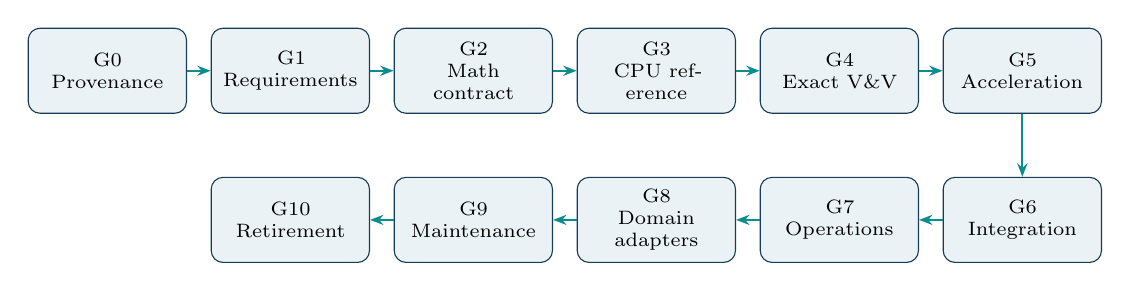
\begin{tikzpicture}[node distance=4mm and 3mm,every node/.style={font=\scriptsize,align=center}]
\tikzset{life/.style={draw=nhdfnavy,rounded corners=1.5mm,fill=nhdflight,text width=1.75cm,minimum height=1.08cm,inner sep=1.3mm}}
\node[life] (n0) {G0\\Provenance};
\node[life,right=of n0] (n1) {G1\\Requirements};
\node[life,right=of n1] (n2) {G2\\Math contract};
\node[life,right=of n2] (n3) {G3\\CPU reference};
\node[life,right=of n3] (n4) {G4\\Exact V\&V};
\node[life,right=of n4] (n5) {G5\\Acceleration};
\node[life,below=8mm of n5] (n6) {G6\\Integration};
\node[life,left=of n6] (n7) {G7\\Operations};
\node[life,left=of n7] (n8) {G8\\Domain adapters};
\node[life,left=of n8] (n9) {G9\\Maintenance};
\node[life,left=of n9] (n10) {G10\\Retirement};
\foreach \a/\b in {n0/n1,n1/n2,n2/n3,n3/n4,n4/n5}{
  \draw[-{Stealth[length=1.7mm]},nhdfteal,thick] (\a.east)--(\b.west);
}
\draw[-{Stealth[length=1.7mm]},nhdfteal,thick] (n5.south)--(n6.north);
\foreach \a/\b in {n6/n7,n7/n8,n8/n9,n9/n10}{
  \draw[-{Stealth[length=1.7mm]},nhdfteal,thick] (\a.west)--(\b.east);
}
\end{tikzpicture}
\caption{Lifecycle gates. Flow runs left-to-right on the first row and right-to-left on the second. An adapter may enter only after the core evidence it depends on exists; retirement remains a designed stage.}
\label{fig:lifecycle}
\end{figure}

\section{Gate G0 -- provenance and claim boundary}
\textbf{Input:} supplied documents and external research. \textbf{Output:} source register, traceability matrix, privacy policy, and disposition classes. \textbf{Pass:} every statement is sourced, reasoned, or labeled hypothesis.

\section{Gate G1 -- requirements and hazards}
Declare shapes, motion class, clearance, units, tolerances, missed-contact cost, false-positive cost, determinism, latency, and caller failure policy. \textbf{Pass:} supported and unsupported profiles are unambiguous.

\section{Gate G2 -- mathematical contract}
Define separation/inclusion objects and valid error/motion bounds. \textbf{Pass:} every no-hit statement has a proof obligation and heuristics have no hidden safety authority.

\section{Gate G3 -- deterministic CPU reference}
Implement the smallest clear semantics. \textbf{Pass:} unit/property tests, reference vectors, schemas, failure preservation, and deterministic replay.

\section{Gate G4 -- robust differential validation}
Use exact/adversarial data and independent implementations. \textbf{Pass:} zero false negatives in the declared profile and bounded TOI error. This release has not passed G4 for triangle meshes.

\section{Gate G5 -- accelerated backend}
Port verified semantics to C++/GPU/other hardware. \textbf{Pass:} equivalence plus measured performance, memory, energy, and failure behavior.

\section{Gate G6 -- application integration}
Add response, rollback, uncertainty, and hardware-in-loop testing. \textbf{Pass:} end-to-end tunneling and failure recovery succeed under realistic timing.

\section{Gate G7 -- deployment and operations}
Add signed releases, configuration control, telemetry, alarms, incident replay, and safe disable. \textbf{Pass:} divergence, overflow, invalid bounds, and unsupported inputs are detected operationally.

\section{Gate G8 -- domain adapters}
Only now map the core into a domain with its own laws. \textbf{Pass:} units, invariants, uncertainty, and baselines are preserved, and operator equivalence is measured.

\section{Gate G9 -- maintenance}
Every predicate, tolerance, compiler mode, queue, and broad-phase change triggers regression evidence. \textbf{Pass:} change record, tests, migration, and rollback exist.

\section{Gate G10 -- retirement}
Freeze unsafe or obsolete backends, migrate callers, archive reproducibility artifacts, revoke deployment, and delete personal/sensor data according to policy. \textbf{Pass:} no silent fallback to discrete endpoint checks.

\chapter{Operations, incident response, and change control}
\section{Runtime telemetry contract}
At minimum, record
\begin{equation}
\{g,\Delta t,N_b,N_c,N_{\rm backend},[t^-,t^+],d_{\min},k,\tau_d,\tau_t,
N_{\rm overflow},N_{\rm unsupported},N_{\rm inconclusive},T_{\rm run},h\}.
\end{equation}
This separates geometry, numerical, resource, and application failures.

\section{Alarm conditions}
\begin{itemize}
  \item any replayed false negative;
  \item repeated inconclusive results at an unacceptable rate;
  \item capacity high-water or overflow;
  \item NaN/Inf or invalid motion/error bound;
  \item CPU/GPU divergence;
  \item unsupported shape/motion entering a safety path;
  \item trace or configuration mismatch.
\end{itemize}

\section{Incident package}
Preserve the exact scene, units, configuration, build and compiler hashes, hardware/runtime versions, certificate, bounded trace, random seed, and caller action. Screenshots or identity metadata are not substitutes for cryptographic and reproducible evidence.

\section{Change categories}
A documentation typo is minor. A change to a tolerance, broad-phase bound, root formula, field interpolation, floating-point mode, queue capacity, tie order, or motion model is correctness-affecting and requires revalidation. A new adapter is not ``just configuration'' if it changes state, units, or invariants.

\small\begin{longtable}{@{}L{0.08\textwidth}L{0.23\textwidth}L{0.10\textwidth}L{0.10\textwidth}L{0.385\textwidth}@{}}
\caption{Risk register summary.}\label{tab:risk-register}\\
\toprule ID & Risk & Severity & Likelihood & Primary mitigation \\ \midrule
\endfirsthead
\toprule ID & Risk & Severity & Likelihood & Primary mitigation \\ \midrule
\endhead
R-001 & False-negative broad phase & Critical & Medium & Use conservative swept bounds; exact dataset; never use learned/parity pruning without verification \\
R-002 & Distance oracle overestimates true separation & Critical & Medium & Require true/conservatively biased distance and calibrated Lipschitz/error bounds \\
R-003 & Closure-speed bound too low & Critical & Medium & Derive per motion/shape; test acceleration/rotation; fail invalid bounds \\
R-004 & Floating-point degeneracy & High & High & Inclusion/exact predicates; scale normalization; adversarial corpus; multiple precision modes \\
R-005 & Iteration or queue exhaustion & High & Medium & Explicit INCONCLUSIVE/CAPACITY\_EXCEEDED; step reduction or robust backend \\
R-006 & Contact response conflated with detection & High & Medium & Separate APIs and certificates; response solver owns impulses/friction \\
R-007 & Parity/golden topology treated as proof & High & High & Keep outside safety authority; mandatory ablations \\
R-008 & GPU fast-math changes signs & Critical & Medium & Predicate-specific compile modes; CPU replay; disable backend on divergence \\
R-009 & Approximate/neural SDF lacks error envelope & Critical & High & Do not certify; add conservative error bound or mesh/exact fallback \\
R-010 & Medical or public-safety overclaim & Critical & Medium & Simulation-only labels, governance, clinical/regulatory evidence gates \\
R-011 & Personal identifiers used as keys & High & Medium & Omit from runtime; use standard cryptography and release hashes \\
R-012 & Domain adapter erases constitutive laws & High & High & Typed adapter contract with units/invariants/baselines \\
\bottomrule
\end{longtable}

% =============================================================================
\part{Separated domain adapters}
% =============================================================================

\chapter{Uniform adapter contract}
\section{Definition}
A domain adapter is
\begin{equation}
\mathcal{A}_d=(X_d,\Phi_d,g_d,E_d,O_d,D_d,I_d,M_d,F_d),
\end{equation}
where $X_d$ is domain state, $\Phi_d$ accepted evolution, $g_d=0$ an event/contact/constraint surface, $E_d,D_d$ encoder/decoder, $O_d$ the implemented operator subset, $I_d$ units and invariants, $M_d$ metrics/baselines, and $F_d$ failures/stops.

A meaningful equivalence claim requires
\begin{equation}
\sup_{x\in\mathcal{D}_d}\left\|D_d\big(\mathcal{N}_{\Delta t}(E_d(x))\big)-\Phi_d^{\Delta t}(x)\right\|_{W_d}\le\epsilon_d
\end{equation}
with calibrated uncertainty and declared domain $\mathcal{D}_d$. Reusing the symbols $\rho$, $\phi$, parity, SDF, or tree does not prove this inequality.

\section{Relationship classes}
\begin{itemize}
  \item \textbf{Literal CCD:} moving geometric bodies and contact.
  \item \textbf{Boundary-event reuse:} a continuous threshold crossing uses bracketing/inclusion logic but is not called geometric collision.
  \item \textbf{Scheduling analogy:} queues, coordinates, and feedback are reused without physical equivalence.
  \item \textbf{Research hypothesis:} no transfer equivalence has yet been demonstrated.
\end{itemize}

\small\begin{longtable}{@{}L{0.16\textwidth}L{0.15\textwidth}L{0.11\textwidth}L{0.23\textwidth}L{0.245\textwidth}@{}}
\caption{Separated domain adapters and evidence gates.}\label{tab:adapters}\\
\toprule Adapter & CCD relationship & Maturity & Next evidence gate & Hard boundary \\ \midrule
\endfirsthead
\toprule Adapter & CCD relationship & Maturity & Next evidence gate & Hard boundary \\ \midrule
\endhead
Graphics and game engines & Literal CCD & D2 executable scaffold & Exact/inclusion CCD datasets; response integration; GPU equivalence & Parity/golden/Klein are optional scheduling metadata \\
Robotics and public safety & Literal CCD & D1 architecture map & Certified motion bounds, sensor uncertainty, safe stop, governance & No automated identity, suspicion, or use-of-force authority \\
Measurement, sensors, actuators & Literal contact plus boundary-event reuse & D1 contract & Traceability, uncertainty budget, actuator dynamics, hardware-in-loop tests & SDF is a calibrated geometric model, not the material itself \\
SAR and wave sensing & Boundary-event reuse & D0-D1 hypothesis & Measured focus metrics against established autofocus baselines & A focus zero set is not a rigid-body collision \\
GPU and edge AI & Scheduling analogy plus literal CCD acceleration & D1 design & Exact replay, no-false-negative broad phase, quality/performance baseline & Learned or parity proposals may not prune safety candidates \\
Optical and photonic computing & Operator-equivalence research & D0-D1 hypothesis & Calibrated transfer error, drift, bandwidth, energy, repeatability & Propagation direction is causal order, not zero latency \\
Quantum and cross-Kerr & Research hypothesis & D0 & Gate/process tomography, noise model, fidelity, classical baseline & Ideal cross-Kerr parity is not assumed in biology or hardware \\
Chemical reaction networks & Boundary-event reuse & D0-D1 hypothesis & Mass/charge balance, calibrated rate laws, reactor experiments & Equilibrium is not automatically an SDF and parity is not universal \\
Biology and medicine & Simulation-only boundary events & D0 & Preclinical/clinical evidence and regulatory pathway for any intervention & No treatment, regeneration, dementia reversal, or crash-immunity claim \\
Fabrication and 3D photonics & Literal geometry checks plus design rules & D1 map & PDK/DRC compliance, optical simulation, metrology, fabricated test coupons & Polar coordinates do not bypass fabrication tolerances \\
Cosmology and holography & Analogy only & D0 & Derive a real duality and compare predictions & SDF boundaries and projection do not establish AdS/CFT-like holography \\
\bottomrule
\end{longtable}

\chapter{Graphics, robotics, measurement, and public safety}
\section{Graphics and game engines}
This is the direct application. The pairwise contact zero set, swept bounds, TOI, witnesses, and response handoff are literal. Version 0.4 supports only a primitive slice, so the next work is robust triangle feature CCD, rotation, deformables, self-collision, simultaneous contacts, and engine response. Recent exact and inclusion datasets provide the required validation foundation \citep{wang2021tight,belgrod2023toi}.

The source projections -- pyramid side, circle, sphere -- become calibration geometry, not guaranteed outputs. Analytic cones may serve as swept support or collision cones, but they must be conservative for the actual shape and motion.

\section{Robotics}
Robot and vehicle planning uses CCD to validate link and environment trajectories. Motion uncertainty, control latency, localization error, and braking distance must enlarge the swept geometry or enter the bound. Hardware-accelerated ray-tracing research is promising for batched robotic collision queries, but representation accuracy and conservative coverage remain explicit tradeoffs \citep{sui2024rtccd}.

\section{Measurement, sensors, and actuators}
The whole-substrate document's broad measurement chain is retained in disciplined form: measurand, transduction, indication, calibration, uncertainty, and interpretation. Metrology terminology and traceability are standardized independently of NHDF \citep{jcgm2012vim}. NHDF may provide a common data/control record, while each sensor retains its transfer function, units, bandwidth, noise, drift, hysteresis, and environment.

CCD is literal for moving stages, shutters, rotors, valves, robotic arms, scanner heads, and mechanical envelopes. For temperature, pressure, or voltage limits, the interval machinery may detect a threshold crossing but should be named boundary-event detection. Actuator response follows electromechanical or material dynamics; parity may request a safety state but is not a restoring force in matter.

\section{Public safety}
A collision engine can support emergency-vehicle navigation, robot safety, mechanical camera rigs, and evidence-device integrity checks. The adapter must not extend geometric prediction into claims of hidden intent or automatic enforcement. Conventional cryptography and chain-of-custody practice, not personal metadata or a geometric phase lock, must secure evidence.

\chapter{SAR, GPU/AI, and wave sensing}
\section{SAR and ionospheric disturbance}
The source maps echo phase and timing residuals into a log-polar LUT, platform motion into kinematics, and focused output into projection. Version 0.4 preserves this as a wave-sensing adapter:
\begin{align}
X_{\rm SAR}&=(s_{\rm echo},x_{\rm nav},\hat\phi_{\rm error}),\\
g_{\rm SAR}(t)&=\text{declared focus or phase-consistency residual}.
\end{align}
A conservative threshold-crossing solver may bracket when the residual leaves an admissible region; bounded trees may partition range, azimuth, scale, or hypotheses. This is not rigid-body collision and does not remove the need for propagation, calibration, autofocus, and image-quality models.

Metrics must include phase RMSE, point-target resolution, peak and integrated sidelobe ratios, image entropy/contrast, compute, memory, dropped frames, and controlled disturbance. ``G3 immunity'' is rejected; the correct behavior is measured degradation, safe mode, stronger integrity codes, and explicit failure.

\section{GPU CCD}
The GPU adapter is a direct acceleration map discussed in Chapter 13. It must preserve every candidate and status. Current CCD work demonstrates both scalable parallel algorithms and the importance of exact validation; the main lesson is that speed and correctness must be measured together \citep{belgrod2023toi}.

\section{Edge AI}
The AI material becomes a separate codec/routing hypothesis. Log-polar coding, local constraints, mixed precision, sparse routing, and bounded feedback may be tested against established quantization, sparsity, and distillation baselines. A learned broad phase may prioritize candidates, but a safety profile cannot allow it to drop pairs unless a conservative verification layer proves the drop safe.

\chapter{Optical, photonic, quantum, and Cross-Kerr adapters}
\section{Optical operator equivalence}
Programmable optics can implement selected linear functions and self-configuring transfer networks \citep{miller2013optical}. The NHDF question is therefore concrete: does a physical transfer $T_{\rm phys}$ reproduce a declared operator $O$ within error,
\begin{equation}
\|T_{\rm phys}(E_{\rm in})-O(E_{\rm in})\|\le\epsilon?
\end{equation}
A first experiment should implement only log-polar encoding plus a local projection or constraint stage. It must report phase/amplitude error, drift, calibration, bandwidth, repeatability, and total energy including conversion.

For CCD, a photonic stage might accelerate a distance transform, convolution, or candidate ranking. It cannot certify no-hit until its worst-case error is conservatively bounded under fabrication variation, temperature, source/detector noise, aging, and calibration failure. A digital verifier should remain in the loop.

\section{Photonic waveguides and direct writing}
Curved and three-dimensional waveguides can be fabricated, but ``native polar geometry'' does not abolish discretization or process windows. A tool path still has finite resolution; optical performance still depends on refractive index, mode confinement, bend loss, roughness, coupling, material absorption, and packaging. The fabrication adapter in Chapter 22 defines the required sequence.

\section{Quantum profile}
A quantum implementation requires state preparation, Hilbert space, Hamiltonian/channel, gates, noise, measurement, readout, and resource scaling. A classical zero-set is not automatically a quantum code. A quantum parity measurement is not the same object as payload XOR parity, topological orientation parity, or CCD root parity.

\section{Cross-Kerr boundary}
The idealized interaction
\begin{equation}
H=\hbar\kappa\hat n_a\hat n_b
\end{equation}
can produce a conditional phase under ideal assumptions. Traveling-wave single-photon gates face response and phase-noise limits; detailed analyses show that causality-induced noise can preclude high-fidelity $\pi$ phase shifts in important regimes \citep{dove2014kerr}. Version 0.4 therefore treats Cross-Kerr parity as a laboratory hypothesis, not as a CCD primitive, a guaranteed chip component, or a biological mechanism.

\chapter{Chemical, biological, and medical adapters}
\section{Chemical reaction networks}
A chemical state is not a geometry word. It is governed by stoichiometry and kinetics, commonly
\begin{equation}
\dot c=S v(c,t),
\end{equation}
with diffusion, temperature, activities, and thermodynamics as required. A concentration threshold or phase boundary $g(c,t)=0$ may use conservative event detection. Log scaling may be useful over wide concentration ranges. A branch graph may represent reactions or compartments.

Programmable BZ-reaction processors demonstrate that hybrid digital-chemical computation is physically real, but they use explicit reactor dynamics, cells, hysteresis, and digital control rather than a universal parity law \citep{sharma2024chemical}. Any NHDF chemical adapter must conserve mass/charge, preserve positivity, calibrate rate laws, and compare with standard solvers and experiments.

\section{Biological modeling}
CCD has direct roles in tissue-tool contact, joint surfaces, catheter navigation, surgical simulation, cells/devices, and anatomical mesh self-collision. Detection must be coupled to biomechanics, fluid dynamics, constitutive behavior, and uncertainty.

Vascular branching is not established as universal golden-ratio scaling. Murray's minimum-work work provides a historically important, assumption-dependent alternative model \citep{murray1926}. Any proposed branching law must be dimensionally valid and tested against data.

\section{Biophotonics}
Ultraweak photon emission is measurable, and theoretical models have proposed myelinated axons as possible optical waveguides \citep{kumar2016myelin}. Disease-model studies have reported altered ultraweak photon activity and spectral shifts \citep{wang2023biophoton,sefati2024upe}. These observations do not demonstrate neural NHDF computation, tubulin photonic-bandgap logic, mitochondrial Cross-Kerr parity, or instant rerouting around damaged tissue.

\section{Medical stop line}
\begin{warningbox}[No therapeutic claim]
This package does not claim to prevent or reverse dementia, regenerate neural tissue, restore swallowing, bypass vascular lesions, stop sepsis, or make an organism immune to failure. A mathematical reparameterization is not an intervention. Any medical claim requires a defined device or treatment, biological mechanism, dose/exposure, toxicology, preclinical replication, clinical trials, ethics, and regulatory review. Current authoritative health information does not support a general dementia cure claim \citep{nia2026dementia}.
\end{warningbox}

\chapter{Fabrication and 3D photonics}
\section{What CCD contributes literally}
CCD can validate moving tool heads, stages, wafer handling, robot paths, and additive-manufacturing trajectories. Static intersection and minimum-separation checks can validate waveguide crossings, ring resonators, electrodes, vias, packages, and curved mask geometry. These are concrete design-rule and motion-planning uses.

\section{What coordinate choice does not remove}
Polar or spherical parameterization may describe rings and spirals efficiently, but fabrication equipment consumes finite-resolution layouts or paths. Process design kits, minimum width/space, etch bias, line-edge roughness, overlay, stitching, material deposition, coupling, thermal drift, and metrology remain. ASML's current High-NA EUV platform is a lithography scanner with 0.55 numerical aperture and an advertised 8 nm resolution; it is not a custom chip designer or complete fab \citep{asml2026highna}.

\section{Credible cradle-to-device sequence}
\begin{enumerate}
  \item define optical/electrical function and process platform;
  \item select materials and a foundry/process design kit;
  \item perform electromagnetic and thermal simulation;
  \item generate curvilinear layout with explicit approximation tolerance;
  \item run design-rule and connectivity checks;
  \item run lithography/process-window simulation where needed;
  \item fabricate test coupons;
  \item measure geometry, loss, phase, bandwidth, and drift;
  \item calibrate the model and repeat;
  \item only then integrate a computing or sensing demonstration.
\end{enumerate}

Direct laser writing can alter the manufacturing route, but it does not ``bypass fabrication'' in the sense of removing materials, equipment, process calibration, packaging, or metrology. It is a different fabrication stack.

\chapter{Cosmology and the limit of the substrate claim}
\section{Holographic word versus holographic principle}
Projection, wavefront processing, or distributed storage may be called holographic in engineering. The holographic principle in quantum gravity is a precise relation between theories, observables, degrees of freedom, entropy, and dynamics; AdS/CFT is the canonical example \citep{maldacena1998}. An SDF boundary and a projection operator do not by themselves establish such a duality.

\section{Permitted use}
CCD and event-surface machinery may appear inside numerical relativity, particle simulation, ray propagation, or astrophysical software. That computational reuse does not imply that spacetime fundamentally executes the NHDF chain. The cosmology adapter remains D0 until it states two theories and derives a testable correspondence or new prediction.

\chapter{Integrated adapter roadmap}
\section{Order of work}
The separate materials should not all advance in parallel at equal priority. A rational sequence is:
\begin{enumerate}
  \item complete triangle/convex/SDF CCD validation;
  \item build a GPU-equivalent backend;
  \item integrate one graphics or robotics application;
  \item test NHDF scheduling ablations;
  \item implement a narrow optical operator-equivalence experiment;
  \item pursue fabrication only after simulation and process rules are selected;
  \item keep chemical, biological, medical, quantum, and cosmological work as independent collaborations with domain specialists and separate evidence plans.
\end{enumerate}

\section{Why this preserves the entire project}
Separating adapters is not a retreat. It gives every domain a common systems contract while preserving the constitutive laws that make the domain real. The shared contribution can be an architecture for constrained state, continuous event detection, bounded routing, observation, and feedback. A universal ontological claim is unnecessary and currently unsupported.

% =============================================================================
\part{Release roadmap, risks, and appendices}
% =============================================================================

\chapter{Version roadmap to 1.0}
\begin{longtable}{@{}L{0.14\textwidth}L{0.24\textwidth}L{0.52\textwidth}@{}}
\caption{Proposed release sequence.}\label{tab:versions}\\
\toprule Version & Center & Exit evidence \\ \midrule
\endfirsthead
\toprule Version & Center & Exit evidence \\ \midrule
\endhead
0.4 & Typed CCD scaffold & Current PDF/ZIP; primitive exact/CA reference; tests; lifecycle and adapters. \\
0.5 & Robust linear triangle CCD & Exact TOI corpus, vertex--face and edge--edge backends, degeneracy catalog, zero false negatives in declared profile. \\
0.6 & Convex and rigid motion & GJK/support mapping or cone casting, rotational bounds, curved trajectory handling, independent differential tests. \\
0.7 & SDF production profile & Certified/biased fields, triangle--SDF and SDF--SDF comparison, rotation, adaptive sampling, error envelopes. \\
0.8 & GPU backend & CPU/GPU equivalence, deterministic mode, overflow equality, measured latency/memory/power. \\
0.9 & Application proof & One graphics/robotics integration outperforming or complementing a selected baseline without correctness regression. \\
1.0 & Stable core & Frozen API, supported profiles, external review, continuous exact-data testing, operations and retirement support. \\
1.x-adapter & Domain-specific & Separate version, domain laws, uncertainty, ethics/regulation, and measured operator equivalence. \\
\bottomrule
\end{longtable}

\section{Definition of done for 1.0}
\begin{itemize}
  \item public supported-profile matrix;
  \item exact and adversarial continuous test service;
  \item independent reproduction on at least two platforms;
  \item complete failure-state and resource semantics;
  \item CPU and accelerated backends with equivalence reports;
  \item stable serialization and API;
  \item one validated application integration;
  \item security, privacy, operations, incident, change, and retirement documentation;
  \item removal or isolation of operators that fail ablations.
\end{itemize}

\chapter{Conclusions}
The earlier work can be made stronger by narrowing its first proof target. CCD provides a literal and demanding realization of the central idea: valid states lie on local constraint surfaces; motion is continuous and causal; swept bounds conservatively restrict work; bounded refinement isolates events; projection emits an observable certificate; and feedback updates the next generation.

The executable v0.4 release demonstrates this architecture for exact linear spheres, sphere--plane contact, swept AABBs, and conditional point/sphere--SDF conservative advancement. It also demonstrates the discipline that a complete engine needs: explicit unsupported cases, initial overlap, inconclusive results, capacity failure, deterministic traces, schemas, tests, benchmarks, and a lifecycle beyond the algorithm.

The source-specific log-polar, parity, phase, golden-ratio, and topology operators remain in the research program, but behind a correctness firewall. They must earn a place through ablation and cannot override geometry. This is the key turn from a broad substrate narrative to a testable computational contribution.

The optical, quantum, chemical, biological, medical, SAR, fabrication, and cosmological material has not been discarded. It has been mapped into independent adapters that preserve domain laws and define what evidence would be required. That separation is the cradle-to-grave foundation for responsible expansion: one verified core, many explicitly bounded adapters, and no silent leap from shared notation to universal physics.

\appendix
\chapter{Normative minimum specification}
An implementation may call itself an NHDF-CCD conforming engine only if:
\begin{enumerate}
  \item it defines continuous step time and monotonic generation semantics;
  \item it defines supported shape and motion profiles;
  \item it defines conservative broad-phase bounds and visible capacity behavior;
  \item every supported pair has a declared exact, conservative, or inclusion backend;
  \item every no-hit result is justified by a valid bound or exact predicate;
  \item it distinguishes hit, no-hit, initial overlap, inconclusive, unsupported, invalid input, and capacity exceeded;
  \item it outputs a TOI point or bracket with tolerance and backend identity;
  \item it separates detection from response;
  \item it bounds iterations, queues, traces, and workspace;
  \item it supports deterministic replay for validation;
  \item it does not let log-polar, parity, golden-ratio, phase, or topology hints suppress candidates or certify outcomes without a separate proof;
  \item it exposes telemetry sufficient to reproduce a failure;
  \item any accelerated backend is compared with a verified semantic reference;
  \item any domain adapter declares state, laws, units, invariants, uncertainty, metrics, and failure conditions.
\end{enumerate}

\chapter{Symbol table}
\begin{longtable}{@{}L{0.22\textwidth}L{0.68\textwidth}@{}}
\caption{Principal symbols.}\\
\toprule Symbol & Meaning \\ \midrule
\endfirsthead
\toprule Symbol & Meaning \\ \midrule
\endhead
$B_i=(S_i,M_i)$ & Body with shape and motion. \\
$t\in[0,1]$ & Normalized time over one proposed simulation step. \\
$\sepfn(t)$ & Pairwise separation or backend-specific contact function. \\
$\TOI$ & Earliest time of impact. \\
$[t^-,t^+]$ & Conservative time-of-impact bracket. \\
$L$ & Valid Lipschitz/closure-speed bound for separation over an interval. \\
$\eta$ & Conservative advancement safety factor in $(0,1]$. \\
$\tau_d,\tau_t$ & Distance and time tolerances. \\
$\SigmaState$ & Complete typed runtime state threaded through operators. \\
$E_{\rm scene}$ & Input validation and encoding. \\
$C_{\rm pair}$ & Conservative broad-phase candidate generation. \\
$B_{\rm bound}$ & Narrow-phase oracle and bound construction. \\
$A_{\rm CA}$ & Conservative advancement. \\
$R_{\rm refine}$ & Exact/inclusion/interval earliest-contact refinement. \\
$\Pi_{\rm cert}$ & Certificate emission. \\
$U$ & Telemetry, cache, and next-generation update. \\
$\rho,\theta$ & Log-separation and approach-direction scheduling coordinates. \\
$\Delta^2\phi$ & Wrapped second finite difference of phase/direction metadata. \\
\bottomrule
\end{longtable}

\chapter{Package manifest overview}
\begin{longtable}{@{}L{0.36\textwidth}L{0.54\textwidth}@{}}
\caption{Top-level ZIP layout.}\\
\toprule Path & Purpose \\ \midrule
\endfirsthead
\toprule Path & Purpose \\ \midrule
\endhead
\texttt{00\_provenance/} & Source register, evidence boundary, privacy/authorship policy, and mounted copies of sources S1--S3; source S4 remains a registered conversation attachment. \\
\texttt{01\_problem\_definition/} & Requirements and release acceptance criteria. \\
\texttt{02\_formal\_specification/} & Typed operator contract, certificate semantics, JSON schemas, and state machine. \\
\texttt{03\_reference\_implementation/} & Python package, examples, C++17 slice. \\
\texttt{04\_verification/} & Tests, adversarial catalog, plan, and bundled verification report. \\
\texttt{05\_benchmarks/} & Deterministic generators, reference vectors, JSON/CSV results. \\
\texttt{06\_gpu\_port\_plan/} & GPU architecture and uncompiled CUDA exact-sphere skeleton. \\
\texttt{07\_integration/} & Engine integration, response boundary, public-safety governance. \\
\texttt{08\_operations/} & Runbook and change control. \\
\texttt{09\_retirement/} & Decommissioning and migration plan. \\
\texttt{10\_domain\_adapters/} & Uniform contract, matrix, and eleven separated adapter documents. \\
\texttt{11\_report/} & LaTeX source, figures, references, generated tables, and final PDF. \\
\texttt{scripts/} & Full verification, benchmark-asset generation, report build, and package hash checks. \\
\texttt{SHA256SUMS.txt} & Hashes for deliverable files after package verification. \\
\bottomrule
\end{longtable}

\chapter{Reproduction commands}
\begin{lstlisting}[language=bash,caption={Full local verification.}]
python -m pip install -e .
pytest
python 05_benchmarks/generate_reference_vectors.py
python 05_benchmarks/run_benchmarks.py
python 11_report/generate_report_assets.py
cmake -S 03_reference_implementation/cpp -B build/cpp \
      -DCMAKE_BUILD_TYPE=Release
cmake --build build/cpp
ctest --test-dir build/cpp --output-on-failure
bash scripts/build_report.sh
python scripts/package_check.py
\end{lstlisting}

The benchmark seed, test files, schemas, and generated reference vectors are included. The external exact TOI datasets and third-party libraries are not redistributed; their project pages and papers are cited for the next validation gate.

\backmatter
\printbibliography[heading=bibintoc,title={References}]

\end{document}
